% OUTLINE version, generated by make_outline.py from report.tex. Numbers come from results/ via report/analysis.py (see notebook/CE893_evaluation.ipynb).
\begin{center}
\vspace*{1.6cm}
{\small CE893-7-AU-CO \textbar{} Generative Artificial Intelligence}\par
\vspace{1.1cm}
{\Huge\bfseries\color{essexpurple}Moving Part of Harness into the Weights:\\[0.2em] Prompt Engineering versus LoRA for a Text-to-Cube Agent}\par
\vspace{0.5cm}
{\Large Fine-tuning (compared with a prompt-engineering harness)}\par
\vspace{1.4cm}
\begin{tabular}{rl}
\textbf{Student name:} & Shamir Dimaano, DIMAA21403
\end{tabular}
\vfill
\end{center}
\clearpage

\section{Introduction and related work}

\subsection{Motivation and context}
\resultplaceholder{\textbf{Write here:}\begin{itemize}[leftmargin=1.2em,itemsep=0.05em]
  \item Who asks: analysts/managers who want a number or a chart, not SQL.
  \item Define semantic layer, cube, dimension, measure (Cube). Why Cube instead of SQL: smaller language, joins handled, rows go straight to a chart.
  \item What is hard: exact member names, dimension vs measure slot, exact stored values, tool order.
  \item The cost of prompting: guide, rules, examples and schema are re-sent on every model call.
\end{itemize}}


\subsection{Related work}
\resultplaceholder{\textbf{Write here:}\begin{itemize}[leftmargin=1.2em,itemsep=0.05em]
  \item Benchmarks: Spider, then BIRD (real databases, evidence hint, execution accuracy).
  \item Prompt-only systems (DIN-SQL) and agent loops (ReAct): our harness is in this family.
  \item Fine-tuned text-to-SQL (CodeS) and API-call fine-tuning (Gorilla).
  \item LoRA and QLoRA make it fit one 16 GB GPU.
  \item Context distillation (Askell et al., Snell et al.): the idea behind moving the prompt into the weights.
\end{itemize}}

\subsection{Research question and contribution}
\resultplaceholder{\textbf{RQ.} When the same agent harness (prompt + tools) is kept fixed, how much does a LoRA adapter trained on verified tool-use transcripts improve execution accuracy on unseen databases, and how much of the prompt (query guide, tool definitions, schema) can the adapter replace without losing accuracy? Questions are asked as an analyst would, without BIRD's hint.}

\resultplaceholder{\textbf{Write here:}\begin{itemize}[leftmargin=1.2em,itemsep=0.05em]
  \item Contribution list: (i) Cube layer + ADK agent for BIRD, (ii) 3,531 execution-verified Cube transcripts from BIRD train, (iii) LoRA adapters for 7B and 14B under three prompt profiles, (iv) demo app (A2UI + Highcharts).
  \item Stress fairness: same Q4\_K\_M model file in Ollama, arms differ only in adapter and prompt.
\end{itemize}}

\begin{figure}[!htbp]
\centering
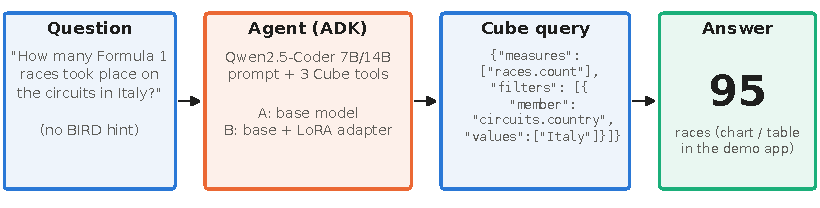
\includegraphics[width=0.7\linewidth]{figures/fig01_glance.pdf}
\caption{Project at a glance. A question goes to the agent, which writes a Cube query; Cube runs it and the rows become the answer (a stat tile here, a chart in the app). The two arms differ only in the LoRA adapter.}
\label{fig:glance}
\end{figure}

\section{Problem definition and proposed solution}

\subsection{Problem definition}
\resultplaceholder{\textbf{Write here:}\begin{itemize}[leftmargin=1.2em,itemsep=0.05em]
  \item One sentence introducing Table 1.
\end{itemize}}
\begin{table}[!htbp]
\centering
\small
\caption{Definition of the task.}
\begin{tabularx}{0.95\linewidth}{@{}lX@{}}
\toprule
\textbf{Element} & \textbf{Definition}\\
\midrule
Intended user & An analyst or manager who asks questions in English about a known database.\\
Input & Question and database name, without BIRD's hint (an analyst would not write one); the harness adds the Cube schema.\\
Required output & One Cube JSON query submitted with \texttt{submit\_answer}; its rows feed the chart.\\
Correct response & The query's rows equal the rows of BIRD's gold SQL on the original SQLite file (order of columns ignored).\\
Constraints & Local model on a 16\,GB GPU; at most 8 model calls per question; only names defined in the Cube models.\\
\bottomrule
\end{tabularx}
\end{table}

\subsection{Proposed solution}
\resultplaceholder{\textbf{Write here:}\begin{itemize}[leftmargin=1.2em,itemsep=0.05em]
  \item Baseline = prompt-engineering harness: guide, rules, 4 examples, schema, 3 tools, pre-checks with 'did you mean' hints (Fig. 2).
  \item Proposed = same harness + LoRA trained on transcripts with exactly this prompt and these tools.
  \item Why fine-tuning fits: output is strict JSON with exact names; baseline errors were format/protocol errors.
\end{itemize}}

\begin{figure}[!htbp]
\centering
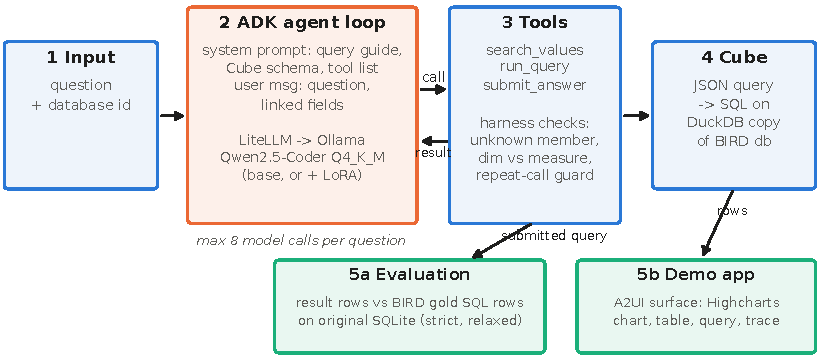
\includegraphics[width=0.76\linewidth]{figures/fig02_pipeline.pdf}
\caption{Steps from input to output. The agent loops between the model and the tools until it submits a query (max.\ 8 calls). The submitted query is scored against the gold SQL (5a) and shown as a chart in the demo app (5b). Every arm uses this same pipeline.}
\label{fig:pipeline}
\end{figure}

\subsection{Expected improvement}
\resultplaceholder{\textbf{Write here:}\begin{itemize}[leftmargin=1.2em,itemsep=0.05em]
  \item Baseline errors on dev data: dimensions in measures, invented members, malformed tool calls.
  \item Expectations: (1) higher accuracy, (2) fewer steps, (3) guide and tool definitions can be dropped once learned.
\end{itemize}}

\section{Data}
\begin{table}[!htbp]
\centering
\small
\caption{Data used. All splits come from BIRD~\cite{li2023bird} (CC BY-SA 4.0). No database appears in more than one split.}
\begin{tabularx}{\linewidth}{@{}l>{\raggedright\arraybackslash}Xrr@{}}
\toprule
\textbf{Split} & \textbf{Purpose} & \textbf{Items} & \textbf{Databases}\\
\midrule
LoRA training & BIRD train questions turned into verified Cube transcripts & 3,273 & 55\\
LoRA validation & Same, three whole databases held out; early-stopping check only & 258 & 3\\
Harness tuning & BIRD dev questions used to develop the prompt and tools & 363 & 3\\
Final test & All BIRD dev questions on \texttt{formula\_1} (174) and \texttt{student\_club} (158); run once per arm & 332 & 2\\
\bottomrule
\end{tabularx}
\end{table}

\subsection{Source and preparation}
\resultplaceholder{\textbf{Write here:}\begin{itemize}[leftmargin=1.2em,itemsep=0.05em]
  \item BIRD fields: question, evidence, gold SQL, SQLite db. Copied to DuckDB; Cube models generated from schema, foreign keys and column descriptions.
  \item Rule-based SQL to Cube translator; keep a pair only if Cube rows = gold rows and non-empty (Fig. 3a funnel: 8,003 to 3,531).
  \item Chat transcript format, loss on assistant turns only; 769 transcripts include a search\_values call.
\end{itemize}}

\begin{figure}[!htbp]
\centering
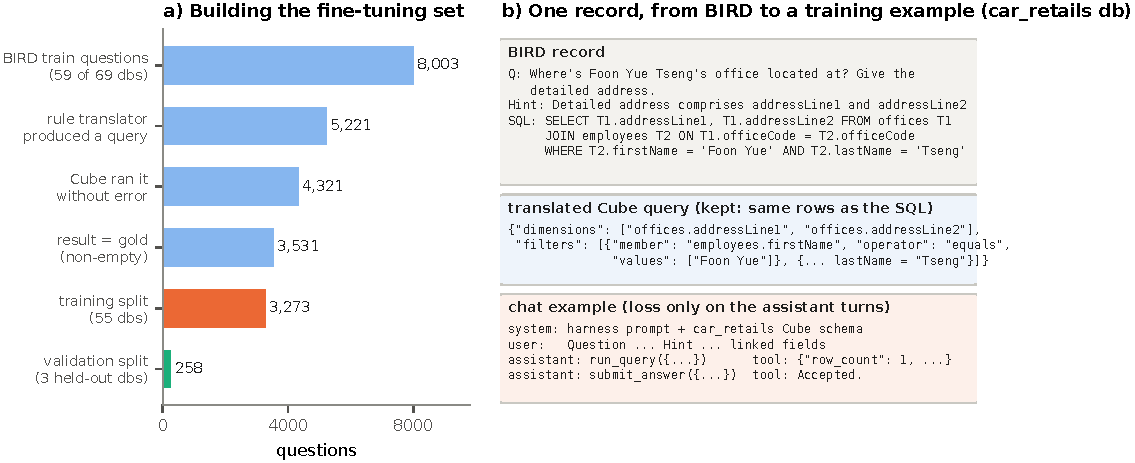
\includegraphics[width=0.78\linewidth]{figures/fig03_data.pdf}
\caption{(a) From 8,003 BIRD training questions to 3,531 verified examples: 2,782 used SQL a semantic layer cannot express, 900 failed in Cube and 790 gave different or empty results. (b) One record, its verified Cube query and the transcript the model is trained on.}
\label{fig:data}
\end{figure}

\subsection{Data quality and limitations}
\resultplaceholder{\textbf{Write here:}\begin{itemize}[leftmargin=1.2em,itemsep=0.05em]
  \item Translator coverage: no subqueries, CASE arithmetic, string slicing; 30\% of test needs such SQL (ceiling 231/332).
  \item BIRD gold SQL has some errors and ties; scoring against gold rows means any correct query counts.
  \item Ten largest training dbs skipped (over 600 MB).
\end{itemize}}

\section{Method}\label{sec:method}

\subsection{Base model and baseline}
\resultplaceholder{\textbf{Write here:}\begin{itemize}[leftmargin=1.2em,itemsep=0.05em]
  \item Qwen2.5-Coder 7B/14B Instruct, Ollama Q4\_K\_M, temperature 0, 16k context.
  \item Harness versions v1 to v4.2 developed on tuning dbs only (Fig. 4); list what each version added; v4.2 frozen before any LoRA run.
\end{itemize}}

\begin{figure}[!htbp]
\centering
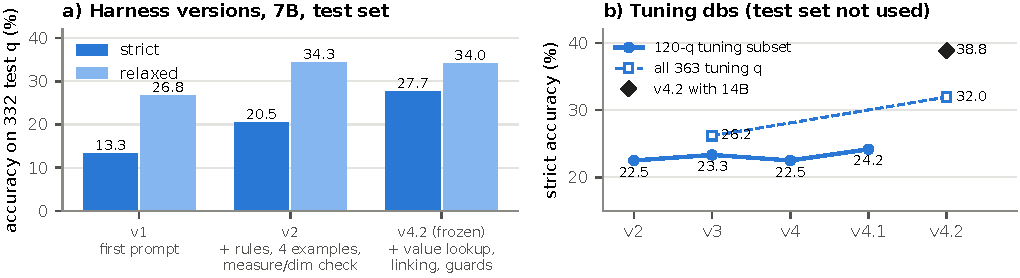
\includegraphics[width=0.8\linewidth]{figures/fig04_harness_versions.pdf}
\caption{Prompt-engineering progress for the 7B baseline (development runs, with BIRD's hint). (a) The three versions that were also run on the test set: strict accuracy doubled from v1 to v4.2. (b) The development loop used only tuning databases; on all 363 tuning questions v4.2 beat v3 (32.0\% vs 26.2\%, McNemar $p{=}0.011$), and the 14B model reached 38.8\%.}
\label{fig:versions}
\end{figure}

\subsection{Chosen method}
\resultplaceholder{\textbf{Write here:}\begin{itemize}[leftmargin=1.2em,itemsep=0.05em]
  \item QLoRA with PEFT: 4-bit NF4 base, rank-16 adapters on all attention + MLP projections (Fig. 5).
  \item Export: merge, GGUF, Q4\_K\_M, base chat template, so only the adapter differs.
  \item Prompt profiles: lean (no guide, no tool schemas, compact schema) and noschema (needs \textasciitilde{}1,300 synthetic questions on the test schemas; no BIRD dev data used).
  \item Fig. 6 (training curves) can be described here or in Results.
\end{itemize}}

\begin{figure}[!htbp]
\centering
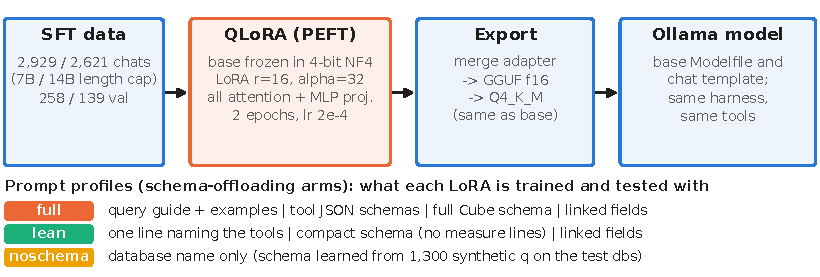
\includegraphics[width=0.75\linewidth]{figures/fig05_method.pdf}
\caption{Fine-tuning pipeline (top) and the three prompt profiles (bottom). Only the adapter and the prompt profile change between arms.}
\label{fig:method}
\end{figure}

\subsection{Implementation details}
\resultplaceholder{\textbf{Write here:}\begin{itemize}[leftmargin=1.2em,itemsep=0.05em]
  \item One sentence introducing Table 3.
\end{itemize}}
\begin{table}[!htbp]
\centering
\small
\caption{Settings needed to reproduce the method.}
\begin{tabularx}{0.95\linewidth}{@{}lX@{}}
\toprule
\textbf{Setting} & \textbf{Value}\\
\midrule
Models & Qwen/Qwen2.5-Coder-7B-Instruct and -14B-Instruct (Hugging Face); Ollama \texttt{qwen2.5-coder:7b/14b} Q4\_K\_M\\
Agent & Google ADK 2.14 \texttt{LlmAgent} via LiteLLM~\cite{adk}; Cube on DuckDB; harness v4.2\\
LoRA & r=16, $\alpha$=32, dropout 0.05, q/k/v/o/gate/up/down projections, 4-bit NF4 base\\
Training & 2 epochs, lr $2\times10^{-4}$ cosine, warm-up 3\%, batch 1 $\times$ 16 accumulation, max.\ 8,192 tokens (7B) / 4,096 (14B, memory limit), seed 7\\
Generation & temperature 0, context 16,384 tokens, at most 8 model calls per question\\
Hardware & one RTX 5070 Ti (16\,GB), 32\,GB RAM, Windows; training 5.3\,h (7B) and 9.0\,h (14B)\\
\bottomrule
\end{tabularx}
\end{table}

\begin{figure}[!htbp]
\centering
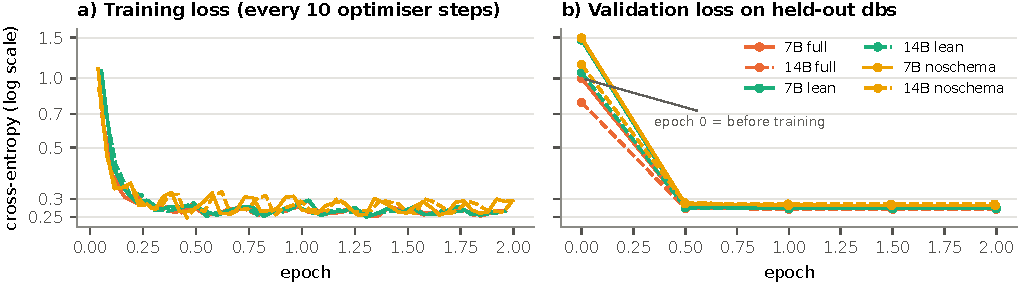
\includegraphics[width=0.78\linewidth]{figures/fig06_training.pdf}
\caption{Training progress for all six adapters. The loss drops within the first quarter epoch and then stays flat; validation loss on the three held-out databases follows it, so the adapters did not overfit. Lean and noschema adapters start higher because the model has never seen those short prompts.}
\label{fig:training}
\end{figure}

\section{Experiments}

\subsection{Compared systems}
\resultplaceholder{\textbf{Write here:}\begin{itemize}[leftmargin=1.2em,itemsep=0.05em]
  \item Baseline: base model + harness v4.2 (full prompt).
  \item Proposed: same model file + LoRA, same harness and prompt.
  \item No-hint runs: baseline and LoRA at both sizes with the hint hidden (adapters were trained with hints).
  \item Prompt-offloading arms: lean LoRA; noschema LoRA with no schema / with lean prompt; control = full LoRA given the lean prompt without retraining.
\end{itemize}}

\subsection{Evaluation data and measures}
\resultplaceholder{\textbf{Write here:}\begin{itemize}[leftmargin=1.2em,itemsep=0.05em]
  \item 332 test questions, 2 unseen dbs, difficulty mix 218/91/23, 77\% need a join. Introduce Table 4.
\end{itemize}}

\begin{table}[!htbp]
\centering
\small
\caption{Evaluation measures.}
\begin{tabularx}{\linewidth}{@{}l>{\raggedright\arraybackslash}X@{}}
\toprule
\textbf{Measure} & \textbf{How it is calculated}\\
\midrule
Strict accuracy (primary) & \% of the 332 questions whose rows and column count equal the gold SQL result\\
Relaxed accuracy & As strict, but extra columns are allowed (Cube must return any dimension it sorts by)\\
Prompt tokens / question & Prompt tokens summed over all model calls of one question\\
Steps, latency, speed & Model calls per question; model seconds per question (mean, median, 90th percentile); output tokens per model second\\
Tool use & Calls per tool, calls the harness or Cube turned back, and answers whose last draft returned no rows\\
Significance & Exact McNemar test on paired per-question outcomes (strict)\\
\bottomrule
\end{tabularx}
\end{table}

\subsection{Experimental procedure}
\resultplaceholder{\textbf{Write here:}\begin{itemize}[leftmargin=1.2em,itemsep=0.05em]
  \item Order: freeze test split + scoring, tune harness on tuning dbs, freeze v4.2, train each adapter once (seed 7), run each arm once.
  \item List what is identical across arms within a size.
\end{itemize}}

\section{Results}

\begin{table}[!htbp]
\centering
\footnotesize
\caption{Main results on the 332 held-out test questions (no hint). Tok./q: prompt tokens per question. $p$: McNemar, strict, against the harness-only arm of the same size.}
\label{tab:main}
\setlength{\tabcolsep}{4pt}
\begin{tabularx}{\linewidth}{@{}Xrrrrcrr@{}}
\toprule
\textbf{System} & \textbf{Strict\,\%} & \textbf{Relax.\,\%} & \textbf{Tok./q} & \textbf{Steps} & \textbf{Latency (s)} & \textbf{Tok./s} & $p$\\
 & & & & & {\scriptsize mean\,/\,med.\,/\,p90} & {\scriptsize output} & \\
\midrule
7B harness only (baseline) & 21.4 & 27.7 & 15,929 & 4.1 & 3.5\,/\,2.3\,/\,6.8 & 121 & --\\
7B LoRA + harness & \textbf{36.7} & \textbf{40.7} & 7,672 & 2.1 & 1.3\,/\,1.2\,/\,1.7 & 104 & $5{\times}10^{-8}$\\
7B lean LoRA & 34.6 & 36.7 & 3,242 & 2.2 & 1.4\,/\,1.2\,/\,1.5 & 110 & $3{\times}10^{-6}$\\
\midrule
14B harness only (baseline) & 27.4 & 35.8 & 11,952 & 3.2 & 4.6\,/\,3.8\,/\,7.0 & 67 & --\\
14B LoRA + harness & \textbf{40.7} & 45.5 & 7,344 & 2.0 & 2.4\,/\,2.3\,/\,3.2 & 61 & $2{\times}10^{-7}$\\
14B lean LoRA & 40.1 & \textbf{46.1} & 2,988 & 2.0 & 2.3\,/\,2.2\,/\,3.3 & 65 & $1{\times}10^{-6}$\\
\bottomrule
\end{tabularx}
\end{table}

\begin{figure}[!htbp]
\centering
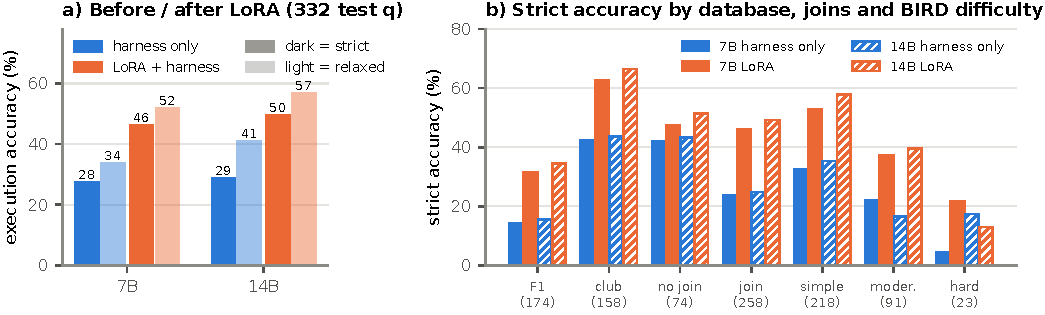
\includegraphics[width=0.68\linewidth]{figures/fig07_main.pdf}
\caption{Before and after fine-tuning (higher is better). (a) The LoRA adds 13--15 points of strict accuracy at both sizes, more than doubling the model size does. (b) The gain holds on both databases and is largest on questions that need a join (7B: 20\% to 35\%, 14B: 23\% to 41\%).}
\label{fig:main}
\end{figure}

\subsection{Main findings}
\resultplaceholder{\textbf{Write here:}\begin{itemize}[leftmargin=1.2em,itemsep=0.05em]
  \item All test runs without BIRD's hint. Lead with Table 5: +15.4 points (7B, 70 fixed vs 19 broken) and +13.3 points (14B, 58 vs 14).
  \item 7B LoRA beats 14B baseline by 9.3 points (p=0.0009); 14B LoRA vs 7B LoRA not significant (p=0.09).
  \item 14B baseline relaxed \textgreater{}\textgreater{} strict (35.8 vs 27.4, extra columns); adapter mostly removes this.
  \item Fig. 8: lean = 1.5k tokens per call vs 3.6k; loses 2.1 (7B, p=0.30) and 0.6 points (14B, p=0.83), n.s. No schema: 18.1\% / 24.7\% (invented members, 114/332 unknown-member errors at 14B); noschema + short schema 37.0 / 41.0. Full LoRA given lean prompt without retraining: 0\%.
\end{itemize}}



\begin{figure}[!htbp]
\centering
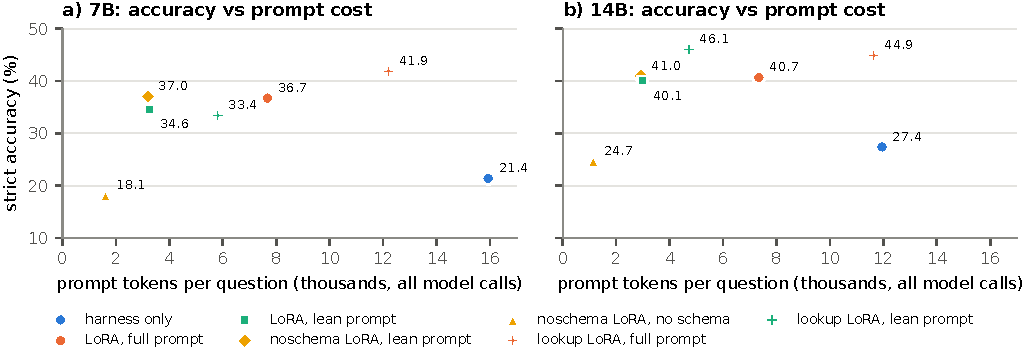
\includegraphics[width=0.74\linewidth]{figures/fig08_offload.pdf}
\caption{Accuracy against prompt cost (up and left is better). The lean adapters (green) match the full LoRA's accuracy at 40\% of its prompt tokens; dropping the schema altogether (triangles) saves more tokens but loses 16--19 points.}
\label{fig:offload}
\end{figure}

\subsection{Tool use}
\begin{table}[!htbp]
\centering
\footnotesize
\caption{Tool use per question (no hint). Lookups: \texttt{search\_values} calls; drafts: \texttt{run\_query} calls; rejected: calls the harness or Cube turned back; text: calls written as text instead of a tool call; empty: answers whose last draft returned no rows.}
\label{tab:tools}
\begin{tabularx}{\linewidth}{@{}Xrrrrrr@{}}
\toprule
\textbf{System} & \textbf{Lookups} & \textbf{Drafts} & \textbf{Rejected} & \textbf{Text \%} & \textbf{No answer \%} & \textbf{Empty \%}\\
\midrule
7B harness only & 1.97 & 0.69 & 1.09 & 16 & 5.4 & 2.4\\
7B LoRA + harness & 0.01 & 1.09 & 0.11 & 0 & 0.0 & 13.0\\
14B harness only & 0.95 & 0.95 & 0.14 & 54 & 0.9 & 10.2\\
14B LoRA + harness & 0.00 & 0.97 & 0.00 & 100 & 0.0 & 13.3\\
\bottomrule
\end{tabularx}
\end{table}

\resultplaceholder{\textbf{Write here:}\begin{itemize}[leftmargin=1.2em,itemsep=0.05em]
  \item Table 6: 7B baseline \textasciitilde{}2 lookups, \textasciitilde{}1 rejected call per q; adapters draft once and submit. But they never look values up: 13\% of answers from an empty draft vs 2-10\%. 14B models write most calls as text.
\end{itemize}}

\subsection{Resource use}
\resultplaceholder{\textbf{Write here:}\begin{itemize}[leftmargin=1.2em,itemsep=0.05em]
  \item Training time 5.3 h (7B), 9.0 h (14B), lean 2-3 h; one 16 GB GPU; converged within half an epoch (Fig. 6).
  \item Steps 4.1 to 2.1, prompt tokens per question halve, model time 3.5 s to 1.3 s (7B), p90 6.8 s to 1.7 s.
  \item Output speed unchanged (\textasciitilde{}105-120 tok/s 7B, 60-67 14B), so the saving is fewer and shorter calls.
  \item Time to first token not measured: future work (would separate prompt processing from decoding).
  \item Caveat: part of the saving is because the adapter skips search\_values (1\% vs 92\%).
\end{itemize}}

\section{Discussion}\label{sec:discussion}

\begin{figure}[!htbp]
\centering
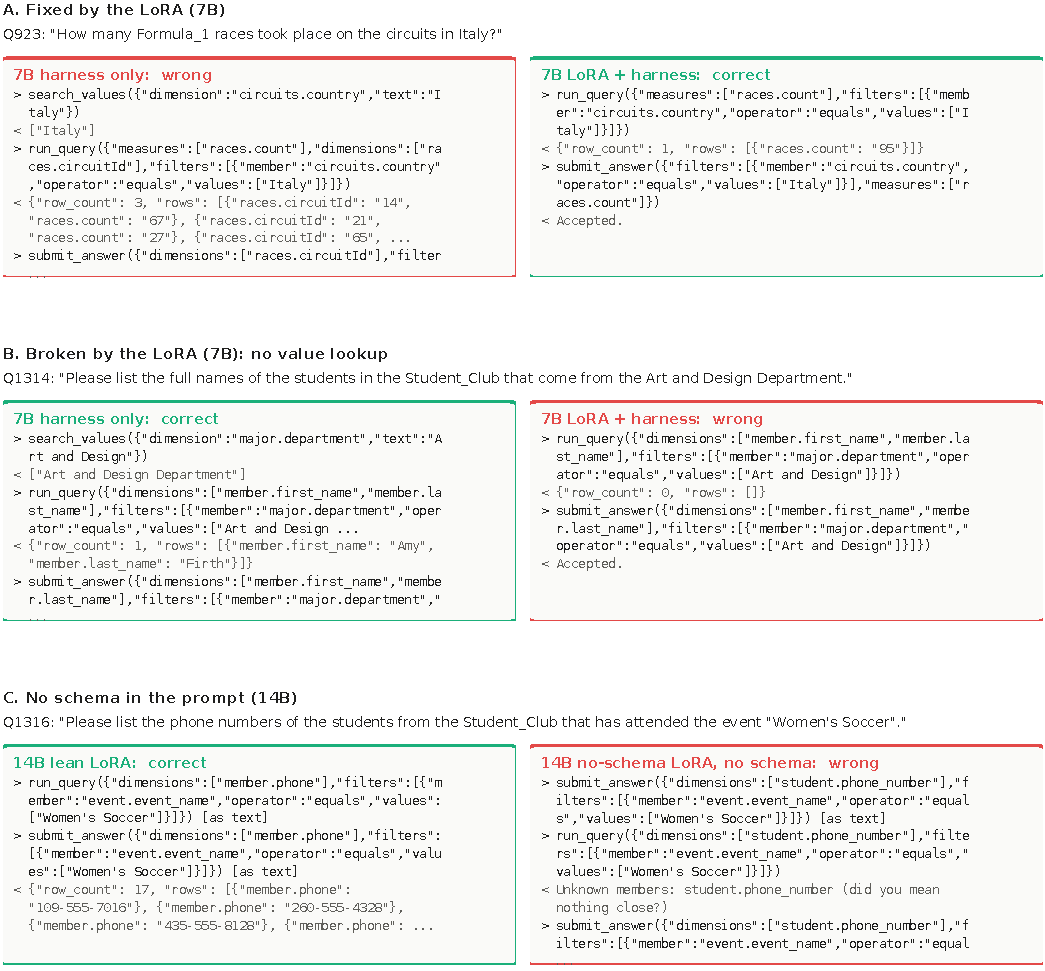
\includegraphics[width=0.7\linewidth]{figures/fig09_outputs.pdf}
\caption{Real tool traces from the test runs (\texttt{>} model call, \texttt{<} tool reply; long lines cut). A: the baseline groups by circuit and returns three rows, the LoRA asks for the single count. B: the LoRA skips the value lookup, filters on a value that does not exist and submits an empty result. C: without a schema the model invents \texttt{student.phone} and repeats it; the lean adapter writes \texttt{member.phone} (here as text, which the harness parses).}
\label{fig:outputs}
\end{figure}

\subsection{Interpretation and error analysis}
\resultplaceholder{\textbf{Write here:}\begin{itemize}[leftmargin=1.2em,itemsep=0.05em]
  \item Walk through Fig. 9 case A (extra grouping dimension) and case B (guessed value, empty result) and case C (invented member without schema).
  \item Fig. 10: failed runs 45 to 4 (7B); wrong filters 64 to 50 (7B), 48 to 39 (14B); \textasciitilde{}55 per arm need SQL Cube cannot express (ceiling, not a model error).
  \item Explain the value-lookup weakness: only 22\% of training transcripts had search\_values.
\end{itemize}}

\begin{figure}[!htbp]
\centering
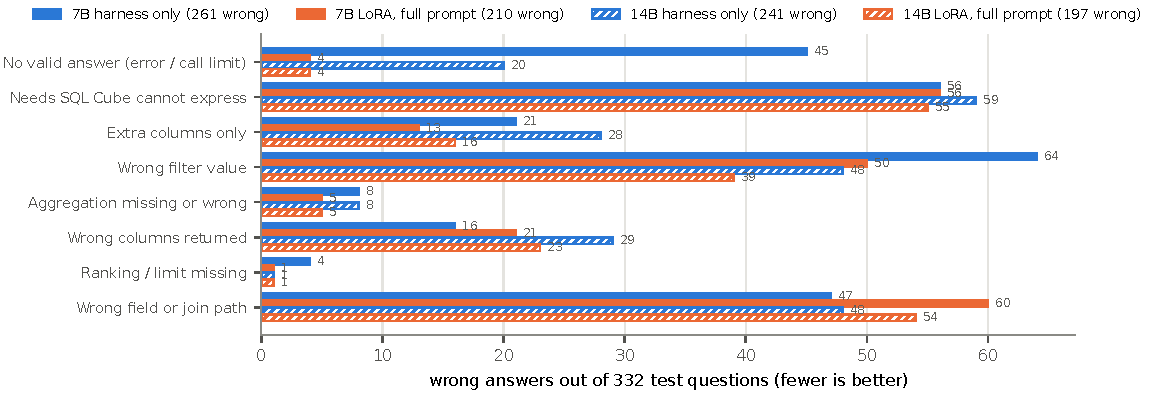
\includegraphics[width=0.62\linewidth]{figures/fig10_errors.pdf}
\caption{Wrong answers by category (rules applied in order). The LoRA mainly removes failed runs, wrong filters and extra columns; about 55 per arm need SQL Cube cannot express.}
\label{fig:errors}
\end{figure}

\subsection{Limitations and responsible use}
\resultplaceholder{\textbf{Write here:}\begin{itemize}[leftmargin=1.2em,itemsep=0.05em]
  \item Two dbs, one run per arm: about $\pm$5 points 95\% interval. With BIRD's hint (standard setting) all arms score higher (LoRA 46.4 / 49.7), so not comparable with leaderboards.
  \item Translator bias toward simple query shapes; noschema is database-specific.
  \item Adapters often write a stray token instead of \textless{}tool\_call\textgreater{} (all 14B calls; also without quantisation); harness parses text calls.
  \item Data: public, no private personal data. Use: wrong filter gives a convincing wrong chart, so the app shows query and trace.
\end{itemize}}

\section{Conclusion}
\resultplaceholder{\textbf{Write here:}\begin{itemize}[leftmargin=1.2em,itemsep=0.05em]
  \item Answer the RQ directly with the two headline numbers and the halved steps.
  \item Most of the prompt can move into the weights (lean within \textasciitilde{}2 points at both sizes, n.s., 40\% of tokens); the schema must stay for unseen dbs.
  \item Main limitation: adapter stopped looking up values.
  \item Future work: search\_values retrain (7B) changed behaviour, not accuracy (36.1 vs 36.7, p=0.88): stray first token -\textgreater{} text fallback, malformed calls. Fix the first-token labels or accept text + JSON; retest; measure time to first token.
\end{itemize}}

{\footnotesize
\let\oldthebibliography\thebibliography
\renewcommand\thebibliography[1]{\oldthebibliography{#1}\setlength{\itemsep}{0.1ex}}
\bibliographystyle{ce893}
\bibliography{references}
}
